\documentclass{standalone}
\usepackage{tikz}
\begin{document}
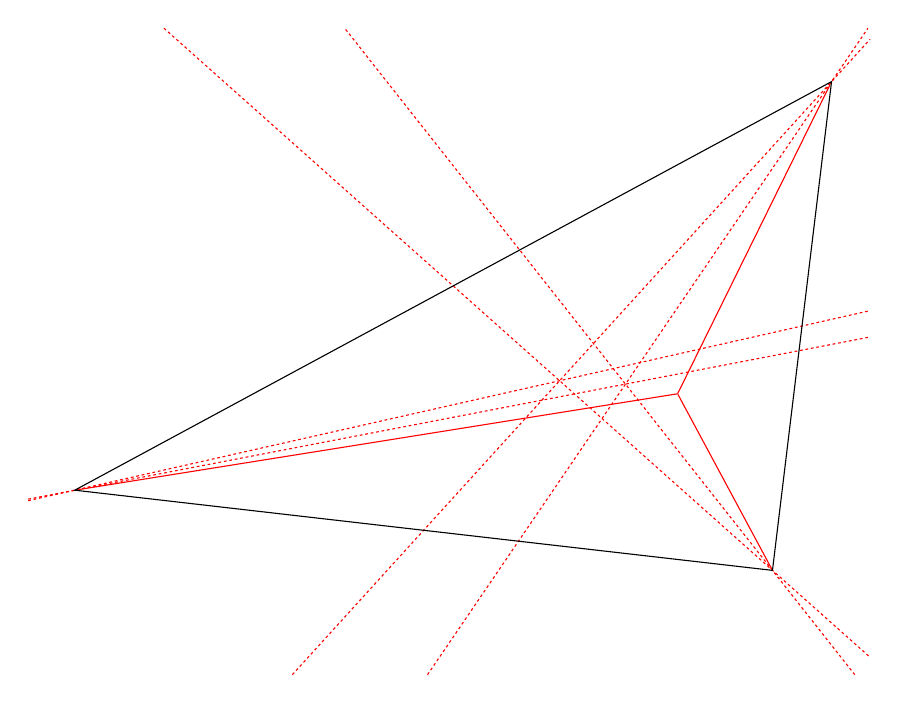
\begin{tikzpicture}[x=1pt,y=1pt]
\draw[red, dash pattern=on 1pt] (296.76,-231.73) -- (112.45,1.87);
\draw[red, dash pattern=on 1pt] (142.38,-231.73) -- (301.51,1.87);
\draw[red, dash pattern=on 1pt] (-1.91,-168.30) -- (302.29,-109.70);
\draw[red, dash pattern=on 1pt] (93.52,-231.73) -- (302.29,-2.11);
\draw[red, dash pattern=on 1pt] (47.13,1.87) -- (302.29,-225.44);
\draw[red, dash pattern=on 1pt] (-1.91,-168.85) -- (302.29,-100.18);
\draw[red] (16.13,-164.87) -- (232.79,-130.21);
\draw[red] (266.77,-193.56) -- (232.85,-130.42);
\draw[red] (232.76,-130.18) -- (287.77,-18.63);
\draw (288.37,-17.42) -- (14.90,-165.06) -- (267.02,-194.03) -- cycle;
\end{tikzpicture}
\end{document}
